\ts\space is a material in the group of \acp{TMD}.
All \ac{TMD} appear in the general form MX\textsubscript{2} with M being a layer of transition-metal atoms such as molybdenum, tungsten or titanium which are sitting between two layers of species X from the group of chalcogens like sulfur or selenium.
This covalently bonded structure is called a \ac{TMD} monolayer.
\Ac{TMD} bulk material is made up of many monolayers stacked monolayers, bonded by van-der-Waals interaction.

The research part of my studies will focus on the \ac{TMD} \ts.
Its crystal structure is depicted in \ref{fig:crystal}\,a. The unit cell contains one titanium atom and two selenium atoms.

\begin{figure}[!t]
	\begin{minipage}{0.5\columnwidth}
		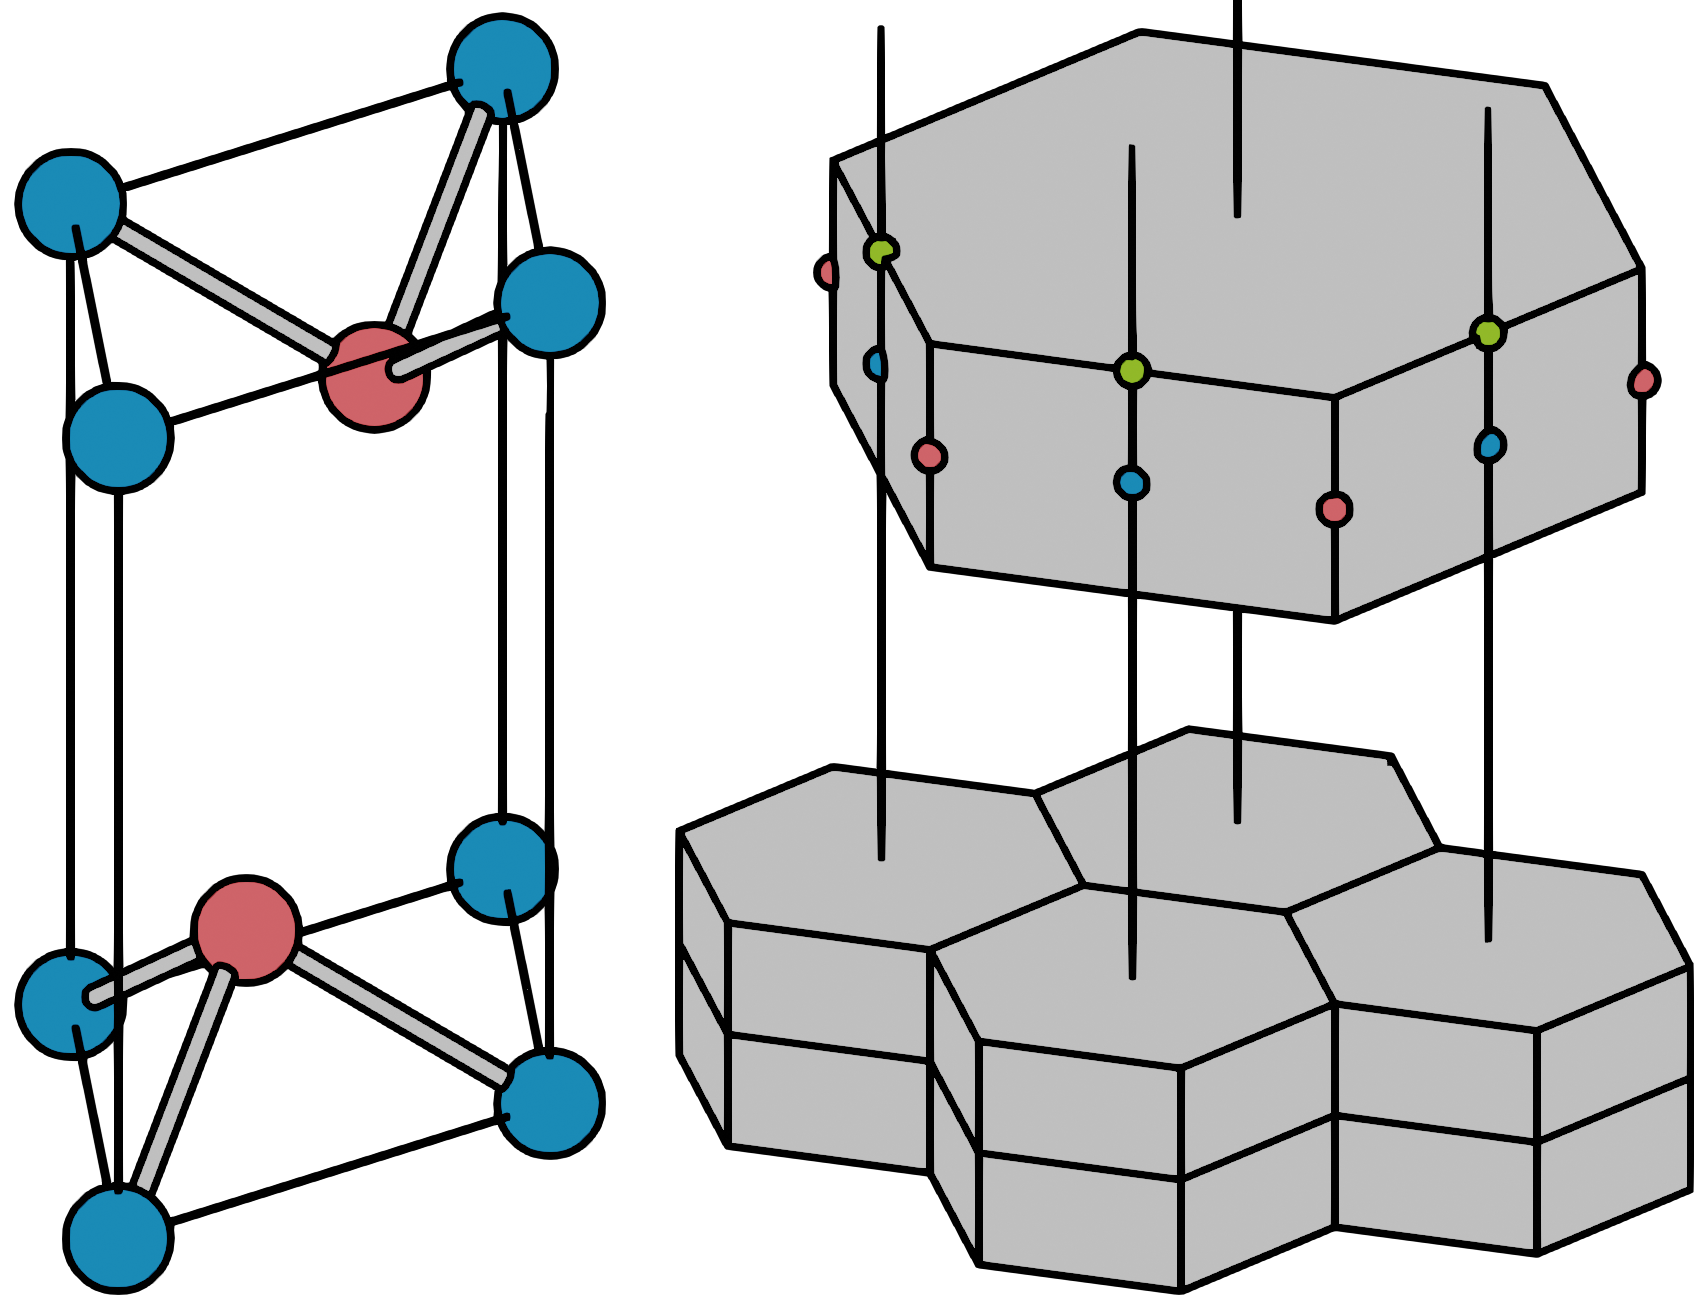
\includegraphics[width=\columnwidth]{figs/tise2_crystal.png}
	\end{minipage}
	\hspace{0.04\columnwidth}
	\begin{minipage}{0.45\columnwidth}
		\caption{a)\,Hexagonal unit cell of \ts, comprised of one Ti atom and two Se atoms. Ti atoms are shown in blue, Se atoms in red. b)\,\ac{BZ} of the high temperature phase (top) and low temperature phase (bottom) of \ts. Blue/red spheres mark M/L points in the \ac{BZ}}
		\label{fig:crystal}
	\end{minipage}
\end{figure}

a = 3.541
c = 6.001
\cite{patel1983}